\documentclass[border=20pt]{standalone}
\usepackage{tikz}
\usetikzlibrary{positioning,arrows.meta}
\begin{document}
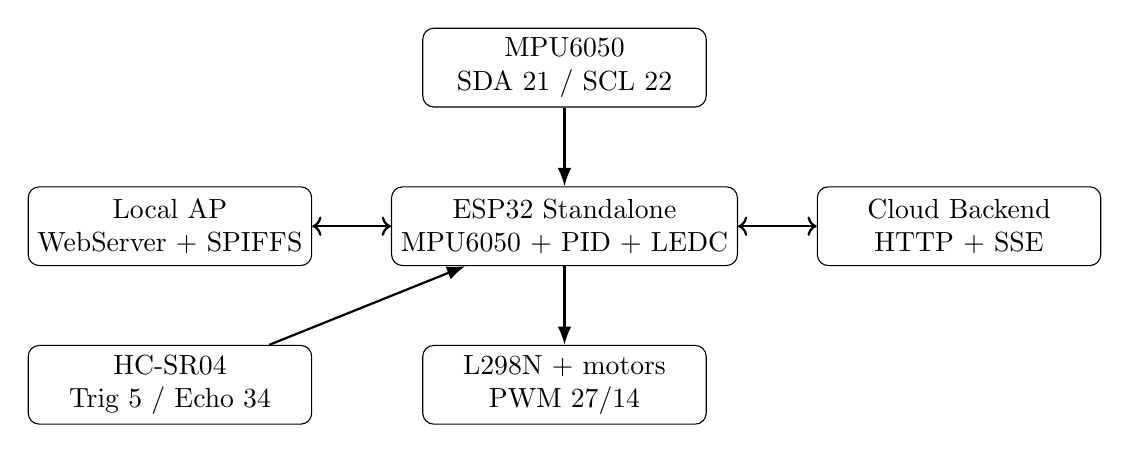
\begin{tikzpicture}[node/.style={draw,rounded corners,align=center,minimum width=3.6cm,minimum height=1cm},line/.style={-Latex,thick}]
\node[node] (e) {ESP32 Standalone\\MPU6050 + PID + LEDC};
\node[node,above=of e] (m) {MPU6050\\SDA 21 / SCL 22};
\node[node,below=of e] (d) {L298N + motors\\PWM 27/14};
\node[node,left=of e] (l) {Local AP\\WebServer + SPIFFS};
\node[node,right=of e] (c) {Cloud Backend\\HTTP + SSE};
\node[node,below left=of e] (s) {HC-SR04\\Trig 5 / Echo 34};
\draw[line] (m)--(e);\draw[line] (e)--(d);\draw[line,<->] (e)--(l);\draw[line,<->] (e)--(c);\draw[line] (s)--(e);
\end{tikzpicture}
\end{document}
